\documentclass{article}

\usepackage{listings}
\usepackage{xcolor}
\usepackage{graphicx}

\newcommand{\BeginThingTaxonomy}{4}
\newcommand{\EndThingTaxonomy}{49}
\newcommand{\BeginAbstractIndividualTaxonomy}{51}
\newcommand{\EndAbstractIndividualTaxonomy}{86}
\newcommand{\BeginEndurantTaxonomy}{88}
\newcommand{\EndEndurantTaxonomy}{145}
\newcommand{\BeginEndurantTaxonomyOfNaturesBegin}{147}
\newcommand{\EndEndurantTaxonomyOfNaturesEnd}{192}
\newcommand{\BeginEndurantTaxonomyOfPropertiesBegin}{194}
\newcommand{\EndEndurantTaxonomyOfPropertiesEnd}{271}
\newcommand{\BeginInstantationAndSpecialzation}{273}
\newcommand{\EndInstantationAndSpecialzation}{356}
\newcommand{\BeginRigidityAndSortality}{360}
\newcommand{\EndRigidityAndSortality}{626}
\newcommand{\BeginEndurantsTypesDefinition}{630}
\newcommand{\EndEndurantsTypesDefinition}{832}
\newcommand{\BeginMereology}{834}
\newcommand{\EndMereology}{885}
\newcommand{\BeginComposition}{887}
\newcommand{\EndComposition}{915}
\newcommand{\BeginConstitution}{917}
\newcommand{\EndConstitution}{935}

\definecolor{codegreen}{rgb}{0,0.6,0}
\definecolor{codegray}{rgb}{0.5,0.5,0.5}
\definecolor{codepurple}{rgb}{0.58,0,0.82}
\definecolor{backcolour}{rgb}{0.95,0.95,0.92}

\lstdefinestyle{mystyle}{
    backgroundcolor=\color{backcolour},
    commentstyle=\color{codegreen},
    keywordstyle=\color{magenta},
    numberstyle=\tiny\color{codegray},
    stringstyle=\color{codepurple},
    basicstyle=\ttfamily\footnotesize,
    breaklines=true,
    keepspaces=true,
    numbers=left,
    numbersep=5pt,
    showspaces=false,
    showstringspaces=false,
    showtabs=false,
    tabsize=2
}

\lstset{style=mystyle}

\title{A TPTP Formalization of the Unified Foundational Ontology}
\author{
    Daniele Porelo,
    Jo\~ao Paulo A. Almeida,
    Giancarlo Guizzardi,\\
    Claudenir M. Fonseca,
    Tiago Prince Sales
}
\date{\today}

\begin{document}
\maketitle

\begin{abstract}
This document presents a formalization of the Unified Foundation Ontology (UFO) expressed in first-order logics through the TPTP syntax. This formalization is intended to support verification of UFO's theory through automated provers and consistency checkers.
\end{abstract}

\section{Introduction}

This document presents a formalization of the Unified Foundation Ontology (UFO) expressed in first-order logics through the TPTP syntax. This formalization is intended to support verification of UFO's theory through automated provers and consistency checkers.

\section{UFO's TPTP Specification}

\subsection{UFO Taxonomy}

% Thing Taxonomy
\subsubsection{Partial Taxonomy of Thing}

\begin{figure}[ht]
    \centering
    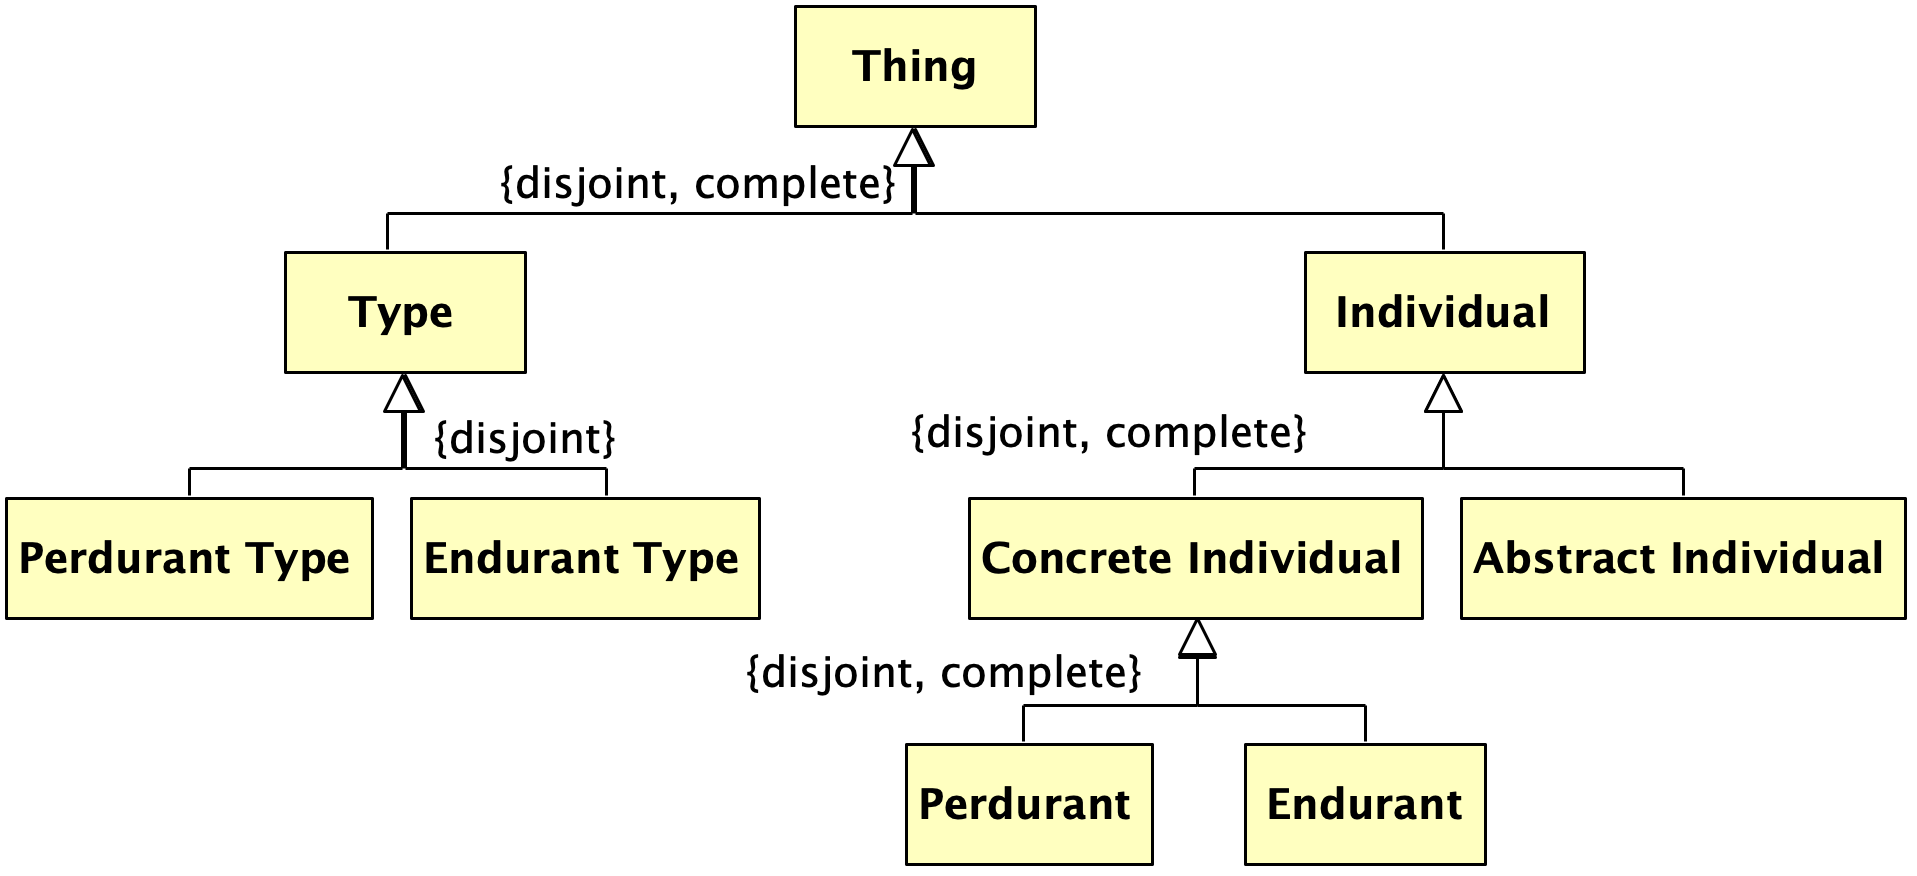
\includegraphics[width=0.8\textwidth]{diagrams/Thing_Diagram.png}
    \caption{Partial Taxonomy of UFO -- Thing.}
    \label{fig:ufo_taxonomy_thing}
\end{figure}

\lstinputlisting[
    firstline=\BeginThingTaxonomy,
    lastline=\EndThingTaxonomy,
    firstnumber=\BeginThingTaxonomy
]{ufo_2021.tex}

% Abstract Individual Taxonomy
\subsubsection{Partial Taxonomy of Abstract Individual}

\begin{figure}[ht]
    \centering
    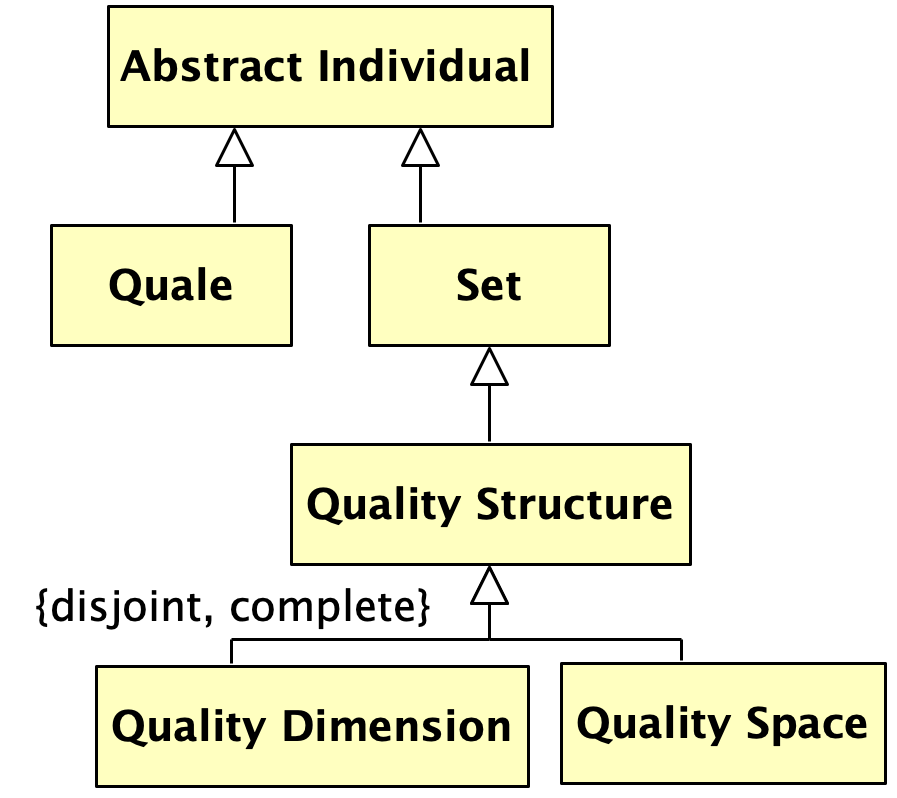
\includegraphics[width=0.4\textwidth]{diagrams/Abstract_Individual_Diagram.png}
    \caption{Partial Taxonomy of UFO -- Abstract Individual.}
    \label{fig:ufo_taxonomy_abstract_individual}
\end{figure}

\lstinputlisting[
    firstline=\BeginAbstractIndividualTaxonomy,
    lastline=\EndAbstractIndividualTaxonomy,
    firstnumber=\BeginAbstractIndividualTaxonomy 
]{ufo_2021.tex}

% Endurant Taxonomy
\subsubsection{Partial Taxonomy of Endurant}

\begin{figure}[ht]
    \centering
    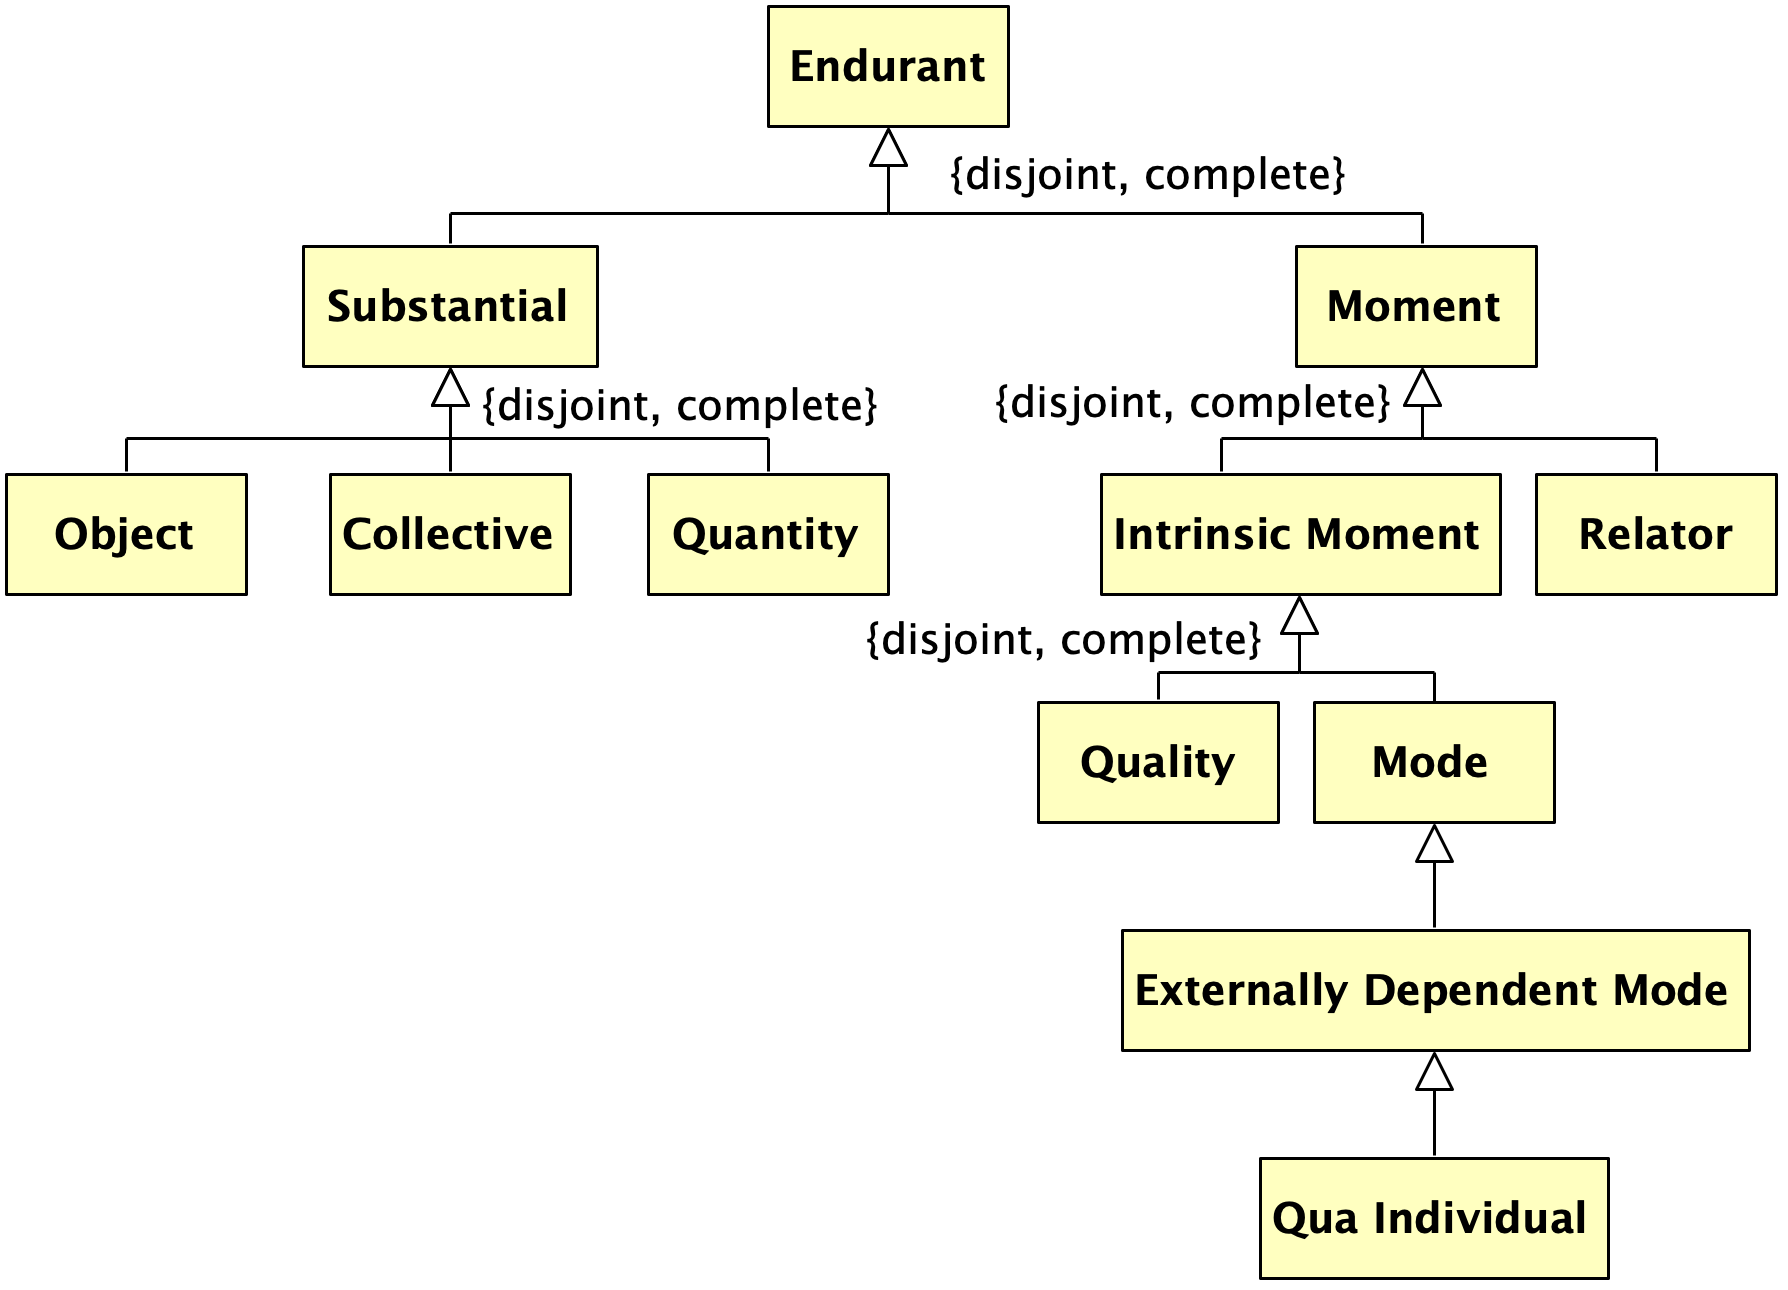
\includegraphics[width=0.8\textwidth]{diagrams/Endurant_Diagram.png}
    \caption{Partial Taxonomy of UFO -- Endurant.}
    \label{fig:ufo_taxonomy_endurant}
\end{figure}

\lstinputlisting[
    firstline=\BeginEndurantTaxonomy,
    lastline=\EndEndurantTaxonomy,
    firstnumber=\BeginEndurantTaxonomy,
]{ufo_2021.tex}

% Endurant Type Taxonomy of Ontological Natures
\subsubsection{Partial Taxonomy of Endurant Type (on ontological natures)}

\begin{figure}[ht]
    \centering
    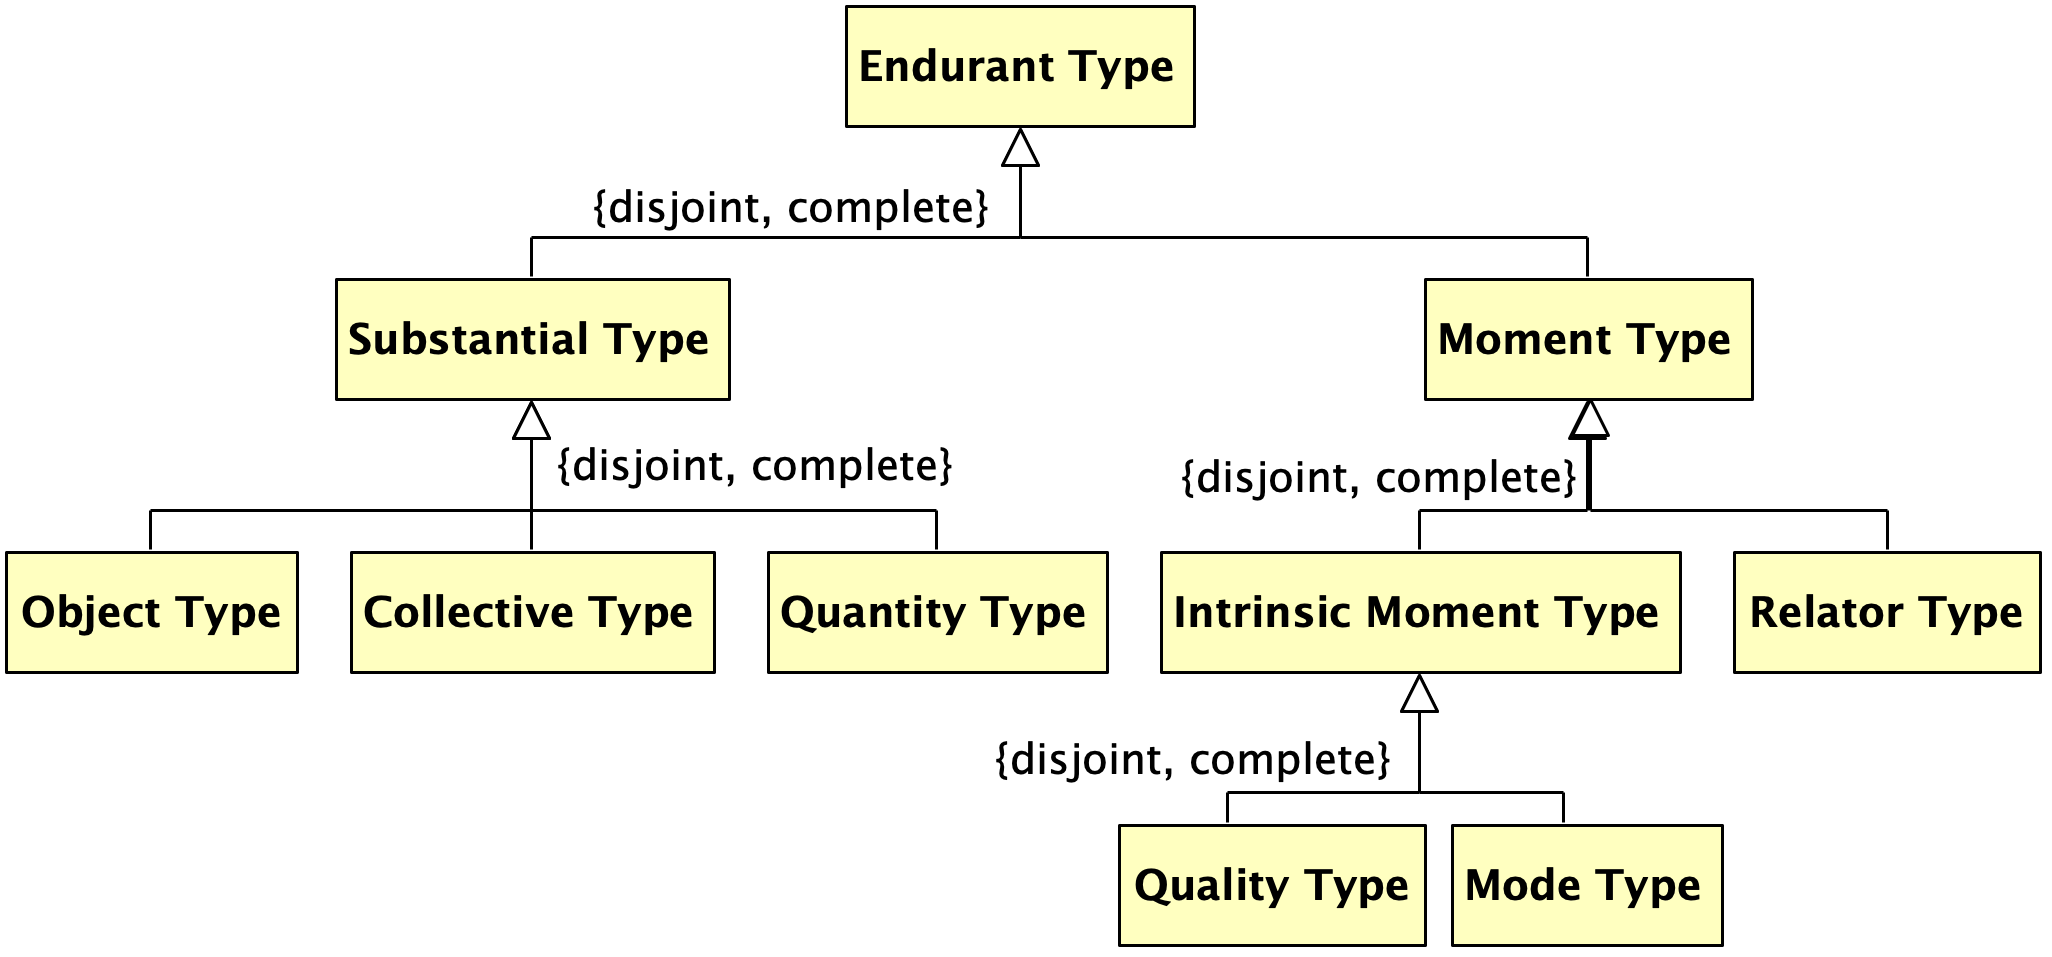
\includegraphics[width=0.9\textwidth]{diagrams/Endurant_Type_Natures_Diagram.png}
    \caption{Partial Taxonomy of UFO -- Endurant Types (by ontological nature).}
    \label{fig:ufo_taxonomy_endurant_types_natures}
\end{figure}

\lstinputlisting[
    firstline=\BeginEndurantTaxonomyOfNaturesBegin,
    lastline=\EndEndurantTaxonomyOfNaturesEnd,
    firstnumber=\BeginEndurantTaxonomyOfNaturesBegin
]{ufo_2021.tex}

% Endurant Type Taxonomy of Modal Properties of Types
\subsubsection{Partial Taxonomy of Endurant Type (on modal properties of types)}

\begin{figure}[ht]
    \centering
    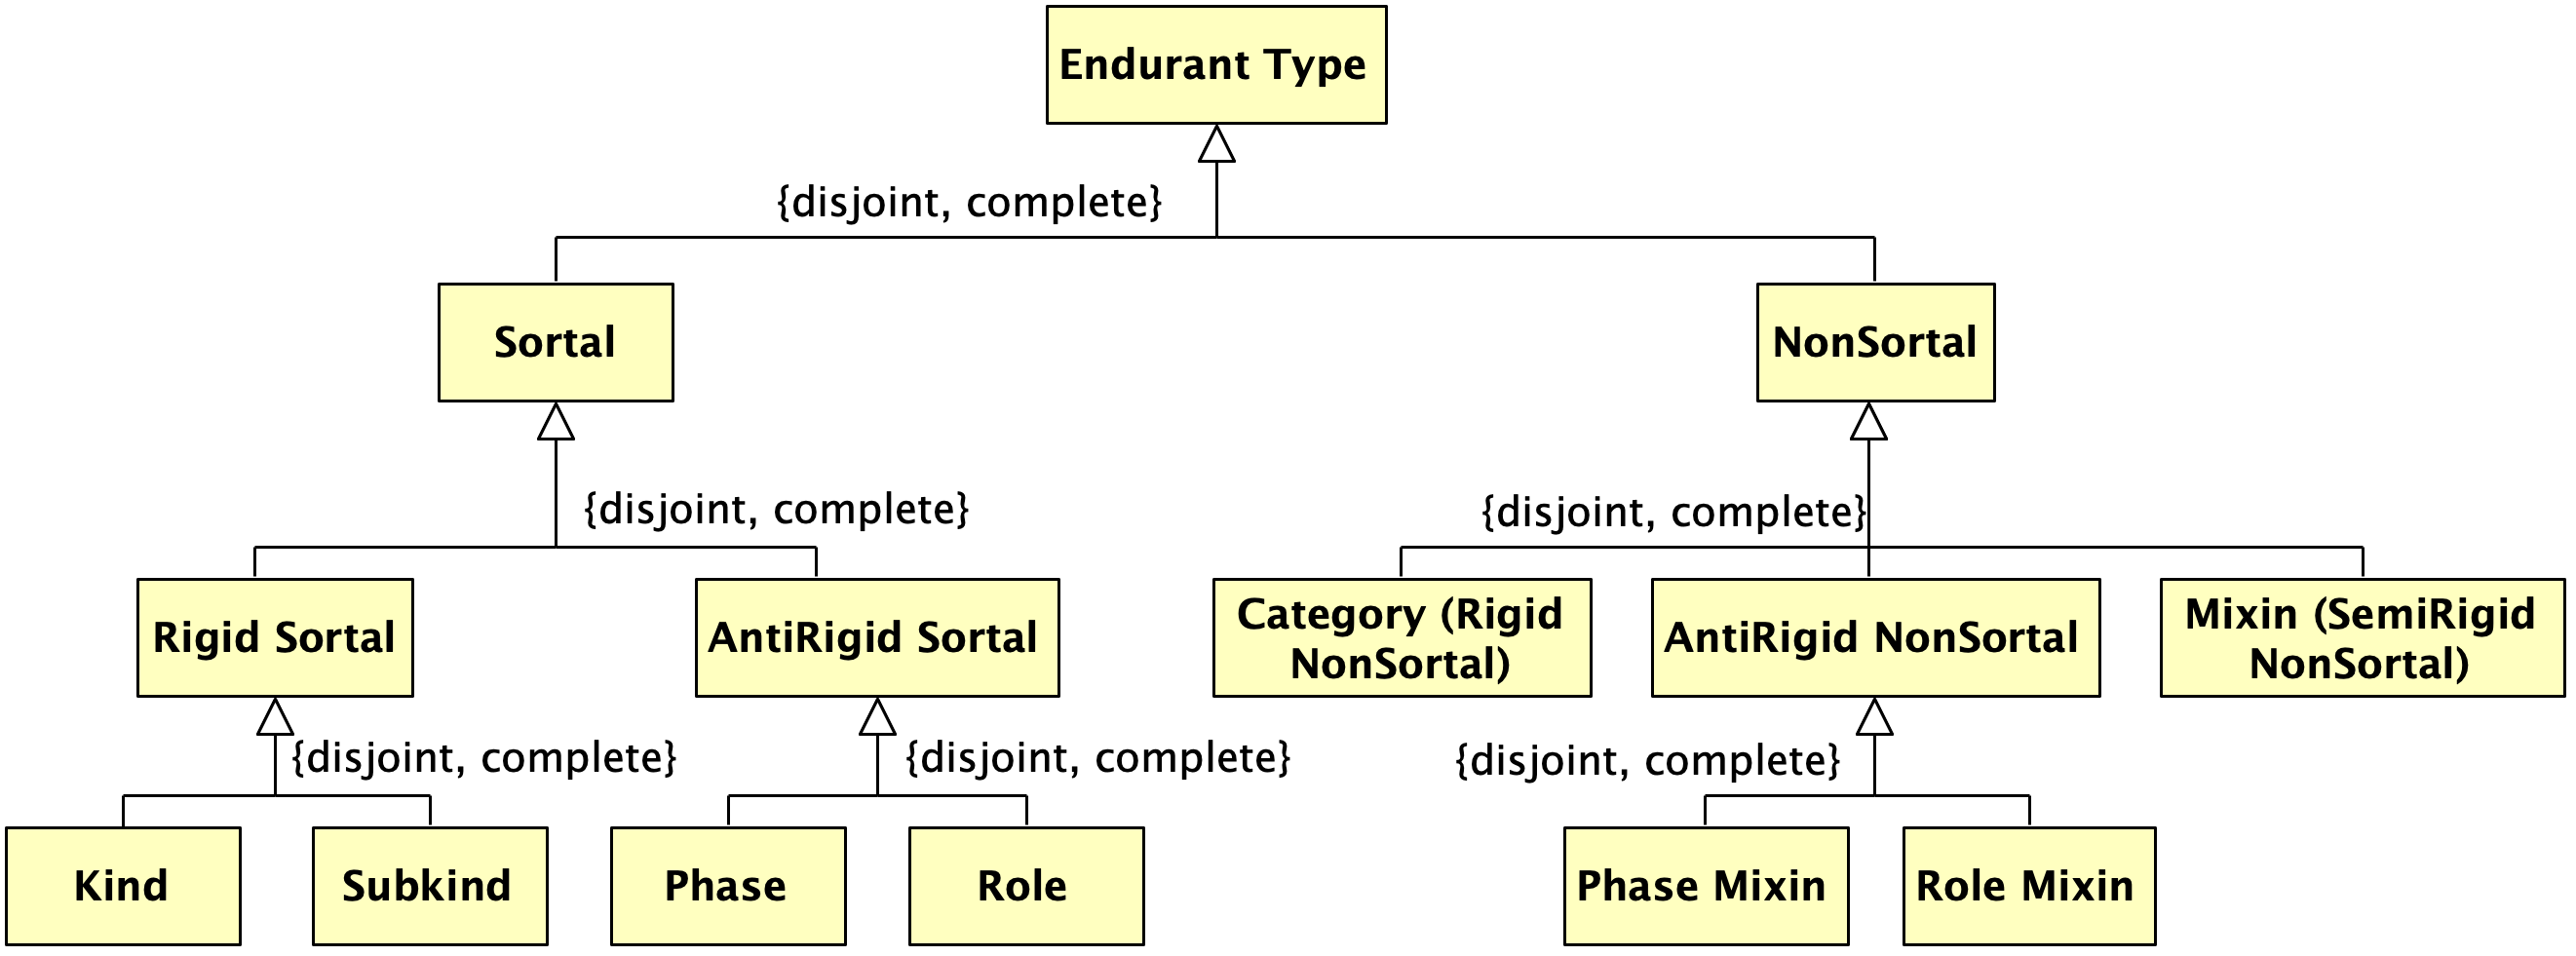
\includegraphics[width=\textwidth]{diagrams/Endurant_Type_Properties_Diagram.png}
    \caption{Partial Taxonomy of UFO -- Endurant Types (by modal properties of types).}
    \label{fig:ufo_taxonomy_endurant_types_properties}
\end{figure}

\lstinputlisting[
    firstline=\BeginEndurantTaxonomyOfPropertiesBegin, 
    lastline=\EndEndurantTaxonomyOfPropertiesEnd, 
    firstnumber=\BeginEndurantTaxonomyOfPropertiesBegin
]{ufo_2021.tex}

% Types, Individuals, Instantiation, and Specialization
\subsubsection{Defining Types, Individuals, and Specialization}

\begin{figure}[ht]
    \centering
    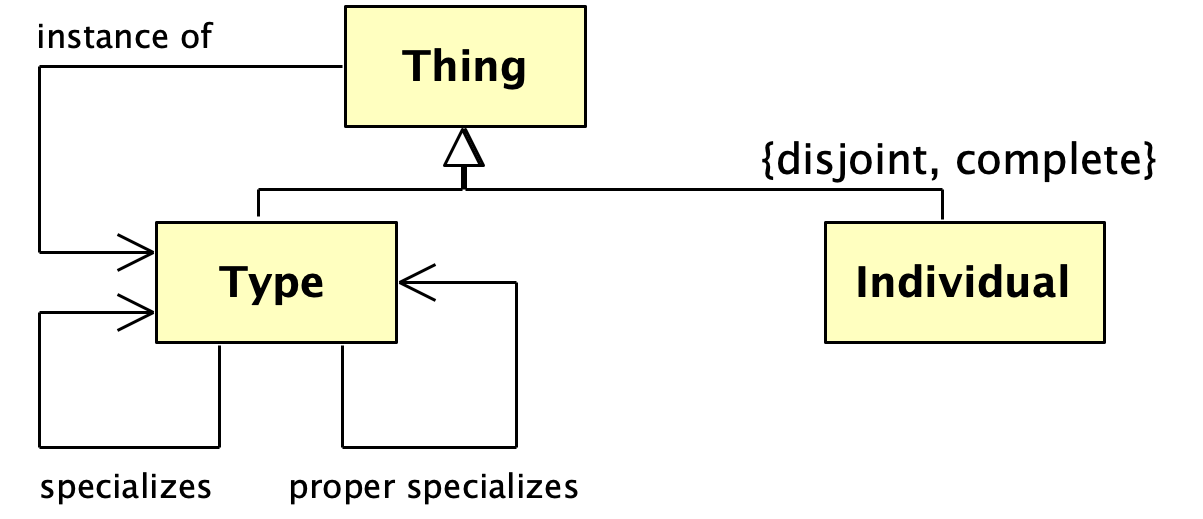
\includegraphics[width=0.6\textwidth]{diagrams/Instantiation_Diagram.png}
    \caption{Types, individuals, instantiation, and specialization.}
    \label{fig:instantiation_and_specialization}
\end{figure}

\lstinputlisting[
    firstline=\BeginInstantationAndSpecialzation, 
    lastline=\EndInstantationAndSpecialzation, 
    firstnumber=\BeginInstantationAndSpecialzation
]{ufo_2021.tex}

% Sortality and Rigidity
\subsubsection{Defining Rigidity and Sortality}

\lstinputlisting[
    firstline=\BeginRigidityAndSortality, 
    lastline=\EndRigidityAndSortality, 
    firstnumber=\BeginRigidityAndSortality
]{ufo_2021.tex}

% Endurant Types Definition
\subsubsection{Defining Endurant Types}

\lstinputlisting[
    firstline=\BeginEndurantsTypesDefinition, 
    lastline=\EndEndurantsTypesDefinition, 
    firstnumber=\BeginEndurantsTypesDefinition
]{ufo_2021.tex}

% Mereology
\subsubsection{Mereology}

\lstinputlisting[
    firstline=\BeginMereology, 
    lastline=\EndMereology, 
    firstnumber=\BeginMereology
]{ufo_2021.tex}

% Composition
\subsubsection{Composition}

\lstinputlisting[
    firstline=\BeginComposition, 
    lastline=\EndComposition, 
    firstnumber=\BeginComposition
]{ufo_2021.tex}

% Constitution
\subsubsection{Constitution}

\lstinputlisting[
    firstline=\BeginConstitution, 
    lastline=\EndConstitution, 
    firstnumber=\BeginConstitution
]{ufo_2021.tex}

% \bibliographystyle{abbrv}
% \bibliography{main}

\end{document}
% This is never printed